\documentclass[12pt]{article}
\usepackage{amsmath, amssymb, amsthm, epsfig}
\usepackage{listings}
\usepackage{fontspec}
\setmonofont{DejaVu Sans Mono}
\usepackage{tikz}
\usetikzlibrary{math,decorations.pathreplacing, shapes.geometric}
\usepackage{quiver}
\usepackage{float}
\usepackage{subcaption}

\usepackage[T1]{fontenc}
\usepackage[utf8]{inputenc}
\usepackage[fixed]{fontawesome5}
\usepackage{pifont}
\usepackage{bbding}

\theoremstyle{definition}
\usepackage{enumitem}
\newenvironment{Proof}{\noindent {\sc Proof.}}{$\Box$ \vspace{2 ex}}
\newenvironment{Solution}{\noindent {\sc Solution.}}{$\Box$ \vspace{2 ex}}


\usepackage{color}
\definecolor{keywordcolor}{rgb}{0.7, 0.1, 0.1}   % red
\definecolor{tacticcolor}{rgb}{0.0, 0.1, 0.6}    % blue
\definecolor{commentcolor}{rgb}{0.4, 0.4, 0.4}   % grey
\definecolor{symbolcolor}{rgb}{0.0, 0.1, 0.6}    % blue
\definecolor{sortcolor}{rgb}{0.1, 0.5, 0.1}      % green
\definecolor{attributecolor}{rgb}{0.7, 0.1, 0.1} % red

\def\lstlanguagefiles{../lstlean.tex}

\oddsidemargin-1mm
\evensidemargin-0mm
\textwidth6.5in
\topmargin-15mm
\textheight8.75in
\footskip27pt

\usepackage[table]{xcolor}
\definecolor{truecolor}{RGB}{198,239,206} % Light green
\definecolor{falsecolor}{RGB}{255,199,206} % Light red
\newcommand{\true}{\cellcolor{truecolor}T}
\newcommand{\false}{\cellcolor{falsecolor}F}
\begin{document}

% homework problems are from the following textbook:
% Larry J. Gerstein, Introduction to Mathematical Structures and Proofs, Undergraduate Texts in Mathematics (https://link.springer.com/book/10.1007/978-1-4614-4265-3)
\noindent \textit{\textbf{Math 300, Winter 2026}} \hspace{1.3cm} \textit{\textbf{HOMEWORK 3}} \hspace{1.3cm} 
\textit{\textbf{Grant Yang}
} 

\vspace{0.5cm}

\begin{Solution}
{\bf (\S2.8, Problem 4)}\\
\begin{enumerate}
    \item $[-2,1]\times[3,5]$: A rectangle spanning from $(-2,3)$ to $(1,5)$:
    \item $\mathbb Z \times \mathbb Z$: A lattice of points at every integer.
    \item $\mathbb Z \times \mathbb R$: An infinite array of vertical lines extending on both directions ($x=n$ on every integer $n$).
    \item $\mathbb R \times \mathbb N$: An array of horizontal lines extending infinitely upwards ($y=n$ on every natural number $n$).
    \item $[1,2]\times \mathbb R$: The graph of $1\le x \le 2$, a strip from $x=1$ to $x=2$ extending infinitely vertically.
    \item $\mathbb N \times [1,2]$: Vertical line segments from $y=1$ to $y=2$ on every natural number for $x$.
\end{enumerate}
Figures are in order left to right. We follow the convention of the book that $0 \not \in \mathbb N$.

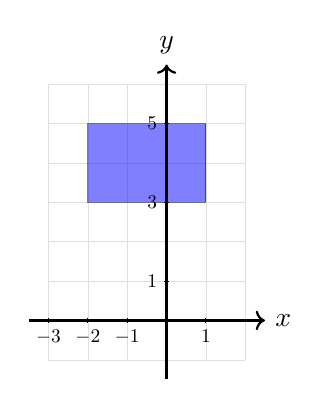
\begin{tikzpicture}[scale=0.5]
    % Draw a light background grid
    \draw[very thin, lightgray!50] (-3,-1) grid (2,6);
    \draw[fill=blue, opacity=0.5] (-2,3) rectangle (1,5);
    % Draw Axes
    \draw[->, thick] (-3.5, 0) -- (2.5, 0) node[right] {$x$};
    \draw[->, thick] (0, -1.5) -- (0, 6.5) node[above] {$y$};

    % Add Tick Labels
    \foreach \x in {-3,-2,-1,1} \draw (\x, 2pt) -- (\x, -2pt) node[below, scale=0.7] {$\x$};
    \foreach \y in {1,3,5} \draw (2pt, \y) -- (-2pt, \y) node[left, scale=0.7] {$\y$};
\end{tikzpicture}
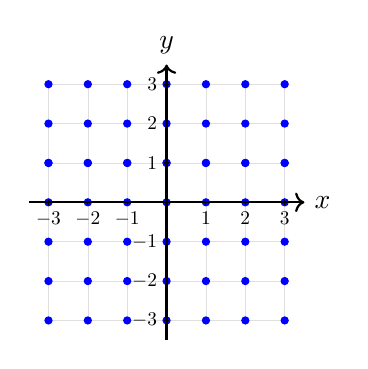
\begin{tikzpicture}[scale=0.5]
    % Draw a light background grid
    \draw[very thin, lightgray!50] (-3,-3) grid (3,3);
    \foreach \x in {-3,-2,-1,0,1,2,3} { \foreach \y in {-3,-2,-1,0,1,2,3,} \fill[blue] (\x, \y) circle (3pt); }
    
    % Draw Axes
    \draw[->, thick] (-3.5, 0) -- (3.5, 0) node[right] {$x$};
    \draw[->, thick] (0, -3.5) -- (0, 3.5) node[above] {$y$};

    % Add Tick Labels
    \foreach \x in {-3,-2,-1,1,2,3} \draw (\x, 2pt) -- (\x, -2pt) node[below, scale=0.7] {$\x$};
    \foreach \y in {-3,-2,-1,1,2,3} \draw (2pt, \y) -- (-2pt, \y) node[left, scale=0.7] {$\y$};
\end{tikzpicture}
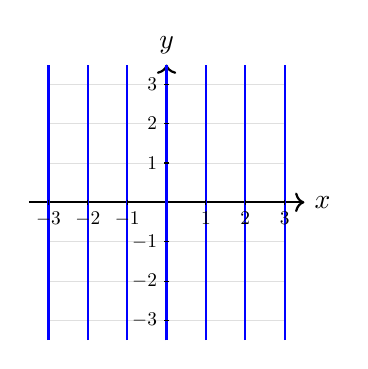
\begin{tikzpicture}[scale=0.5]
    % Draw a light background grid
    \draw[very thin, lightgray!50] (-3,-3) grid (3,3);
    
    % Draw Axes
    \draw[->, thick] (-3.5, 0) -- (3.5, 0) node[right] {$x$};
    \draw[->, thick] (0, -3.5) -- (0, 3.5) node[above] {$y$};
    \foreach \x in {-3,-2,-1,0,1,2,3} { \draw[blue,thick] (\x, -3.5) -- (\x, 3.5); }

    % Add Tick Labels
    \foreach \x in {-3,-2,-1,1,2,3} \draw (\x, 2pt) -- (\x, -2pt) node[below, scale=0.7] {$\x$};
    \foreach \y in {-3,-2,-1,1,2,3} \draw (2pt, \y) -- (-2pt, \y) node[left, scale=0.7] {$\y$};
\end{tikzpicture}
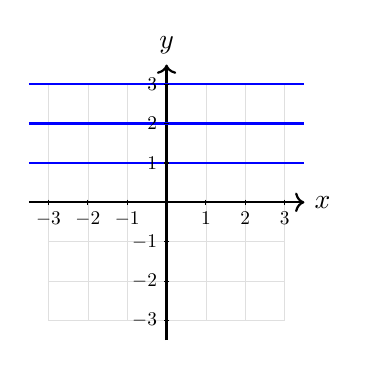
\begin{tikzpicture}[scale=0.5]
    % Draw a light background grid
    \draw[very thin, lightgray!50] (-3,-3) grid (3,3);
    
    % Draw Axes
    \draw[->, thick] (-3.5, 0) -- (3.5, 0) node[right] {$x$};
    \draw[->, thick] (0, -3.5) -- (0, 3.5) node[above] {$y$};
    \foreach \y in {1,2,3} { \draw[blue,thick] (-3.5, \y) -- (3.5, \y); }

    % Add Tick Labels
    \foreach \x in {-3,-2,-1,1,2,3} \draw (\x, 2pt) -- (\x, -2pt) node[below, scale=0.7] {$\x$};
    \foreach \y in {-3,-2,-1,1,2,3} \draw (2pt, \y) -- (-2pt, \y) node[left, scale=0.7] {$\y$};
\end{tikzpicture}
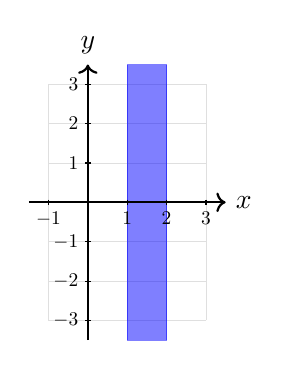
\begin{tikzpicture}[scale=0.5]
    % Draw a light background grid
    \draw[very thin, lightgray!50] (-1,-3) grid (3,3);
   \draw[fill, blue, opacity=0.5] (1,-3.5) rectangle (2, 3.5);
    
    % Draw Axes
    \draw[->, thick] (-1.5, 0) -- (3.5, 0) node[right] {$x$};
    \draw[->, thick] (0, -3.5) -- (0, 3.5) node[above] {$y$};

    % Add Tick Labels
    \foreach \x in {-1,1,2,3} \draw (\x, 2pt) -- (\x, -2pt) node[below, scale=0.7] {$\x$};
    \foreach \y in {-3,-2,-1,1,2,3} \draw (2pt, \y) -- (-2pt, \y) node[left, scale=0.7] {$\y$};
\end{tikzpicture}
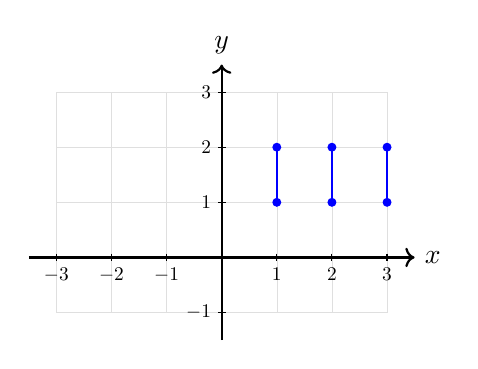
\begin{tikzpicture}[scale=0.7]
    % Draw a light background grid
    \draw[very thin, lightgray!50] (-3,-1) grid (3,3);
    
    % Draw Axes
    \draw[->, thick] (-3.5, 0) -- (3.5, 0) node[right] {$x$};
    \draw[->, thick] (0, -1.5) -- (0, 3.5) node[above] {$y$};
    \foreach \x in {1,2,3} { \draw[blue,thick] (\x, 1) -- (\x, 2); \draw[blue,fill] (\x, 1) circle (2pt) (\x, 2) circle (2pt); }

    % Add Tick Labels
    \foreach \x in {-3,-2,-1,1,2,3} \draw (\x, 2pt) -- (\x, -2pt) node[below, scale=0.7] {$\x$};
    \foreach \y in {-1,1,2,3} \draw (2pt, \y) -- (-2pt, \y) node[left, scale=0.7] {$\y$};
\end{tikzpicture}
\end{Solution}

\vspace{0.5cm}

\begin{Solution}
{\bf (\S2.8, Problem 6)}\\
Define $(a_1,a_2,a_3)=((a_1,a_2),a_3)$. From Theorem 2.40, we know that $(a,b)=(c,d)\iff a=c\land b=d$. For a proof of the forward direction, we can unfold the definition of ordered pair: $(a,b)=(c,d)$ can be rewritten as $\{\{a\},\{a,b\}\}=\{\{c\},\{c,d\}\}$. First consider the case where $a=b$: then we have $\{\{a\}\}=\{\{c\},\{c,d\}\}$, which implies that $\{c\}=\{c,d\}$ and thus $d=c$ since $\{c,d\}$ is a singleton, so we have $d=c=a=b$ as desired. Now consider $a\ne b$. Then $\{a\}\ne\{a,b\}$ as $b\in \{a,b\}$ but $b\not\in\{a\}$. By the original set equality, we must have $\{c\}\in\{\{a\},\{a,b\}\}$. However, $\{c\}\ne\{a,b\}$ since by set equality, $\{c\}=\{a,b\}$ would imply that $a\in \{c\}$ and $b\in \{c\}$ and thus $a=b=c$, which is a contradiction with $a\ne b$. Thus, we must have $\{c\}=\{a\}$ and thus $a=c$. We also must have $\{a,b\}\in \{\{c\},\{c,d\}\}$ by the original set equality, and since $\{a,b\}\ne \{c\}$, we know this must mean $\{a,b\}=\{c,d\}$. Rewriting with $a=c$, this becomes $\{a,b\}=\{a,d\}$, so $d\ne a$ and $d\in \{a,b\}$, which means $d=b$ as desired.
\begin{enumerate}
    \item If $(a_1,a_2,a_3)=(b_1,b_2,b_3)$, we have that $\forall(i\in\{1,2,3\}), a_i=b_i$. We can unfold the definition of 3-tuple and obtain $((a_1,a_2),a_3)=((b_1,b_2),b_3)$. By theorem 2.40, we have $a_3 = b_3$ as desired, and we also have $(a_1,a_2)=(b_1,b_2)$. Applying theorem 2.40 again, we obtain $a_1 =b_1$ and $a_2 = b_2$, completing the proof.
    \item Define an ordered quadruple (aka a 4-tuple) to be $(a_1,a_2,a_3,a_4)=((a_1,a_2,a_3),a_4)$. If $(a_1,a_2,a_3,a_4)=(b_1,b_2,b_3,b_4)$, we have by definition that $((a_1,a_2,a_3),a_4)=((b_1,b_2,b_3),b_4)$. By theorem 2.40, we have $a_4=b_4$ and $(a_1,a_2,a_3)=(b_1,b_2,b_3)$. By our previous result on ordered triples, we have that $\forall(i\in\{1,2,3\}),a_i=b_i$, but since we now have $a_4=b_4$, we can extend this to be $\forall(i\in\{1,2,3,4\}),a_i=b_i$. Thus, our definition satisfies the desired property.
\end{enumerate}
\end{Solution}

\vspace{0.5cm}

\begin{Solution}
{\bf (\S2.9, Problem 5)}\\
\begin{enumerate}
    \item Let $S=\{1,2,3,4,5,6\}$. The following partitions $\Pi_1,\Pi_2,\Pi_3,\Pi_4$ are such that $\Pi_i$ is finer than $\Pi_{i+1}$ for $i\in\{1,2,3\}$.
    \begin{align*}
        \Pi_1 =\{\{1\},\{2\},\{3\},\{4\},\{5\},\{6\}\} &\qquad \Pi_2 = \{\{1,2\},\{3,4\},\{5,6\}\} \\
        \Pi_3 = \{\{1,2,3,4\},\{5,6\}\} &\qquad \Pi_4=\{\{1,2,3,4,5,6\}\}
    \end{align*}
    \item Now considering $\mathbb N$. The following is another chain of partitions such that $\Pi_i$ is finer than $\Pi_{i+1}$.
    \begin{align*}
        \Pi_1 &= \{\{n\} \mid n \in \mathbb N\} \\
        \Pi_2 &= \{\{4n,4n+2\} \mid n \in \mathbb N\} \cup \{\{4n+1,4n+3\} \mid n\in \mathbb N\} \\
        \Pi_3 &= \{\{2n\mid n\in \mathbb N\},\{2n+1\mid n\in \mathbb N\}\} \\
        \Pi_4 &= \{\mathbb{N}\}
    \end{align*}
    \item Let $S$ be a set and let $\Pi =\{A_i\}_{i\in S}$ be a partition of $S$ where $A_s = \{s\}$. $\Pi$ is a partition as $\forall i,A_i\ne \varnothing$, and $\forall i,j \in S, i\ne j \implies A_i \cap A_j = \varnothing$. Further, we can also see that $\bigcup_{i\in S} A_i=\bigcup_{i\in S}\{i\}=\{i\mid i \in S\}=S$. Let $\Pi'=\{B_i\}_{i\in I}$ be any other partition. Then we can show that $\Pi$ is finer than $\Pi'$, i.e. that $\forall (s\in S),\exists(i\in I),A_s \subseteq B_i$. Consider any index $s\in S$. We have the singleton $A_s =\{s\}$, and so by the definition of subset we have that $\forall U,A_s\subseteq U\iff s\in U$. Thus, to prove our claim we only need to show that $\exists (i\in I), s\in B_i$. Consider the property on partitions that $\bigcup_{i\in I} B_i = S$. By construction, we have that $s \in S$, and so $s \in \bigcup_{i\in S} B_i$. However, by the definition of the union of an indexed family of sets, this is exactly the statement that we are trying to prove, $\exists (i\in I), s\in B_i$. For all partitions $\Pi'$ of $S$, $\Pi$ is finer than $\Pi'$.
\end{enumerate}
\end{Solution}

\vspace{0.5cm}

\begin{Solution}
{\bf (\S2.9, Problem 8)}\\
Let $R$ be a relation on $S$. We define $R_1$ to be the symmetric closure of $R$, such that $R_1 \supseteq R$, $R_1$ is symmetric ($\forall (x,y),[xRy\implies yRx]$), and no proper subset of $R_1$ contains $R$. Let $S=\{1,2,3,4\}$ and $R=\{(1,2),(1,3),(2,3),(1,4),(4,1)\}$. The symmetric closure is given by
$R_1 =\{(1,2),(2,1),(1,3),(3,1),(2,3),(3,2),(1,4),(4,1)\}.$
\end{Solution}

\vspace{0.5cm}

\begin{Solution}
{\bf (\S2.9, Problem 10)}\\
Let $C$ be a set of $n$ cities. We define a relation $xRy$ on $x,y\in C$ to be true whenever there is a direct road from $x$ to $y$ that passes through no other cities along the way.

\begin{enumerate}
    \item Assuming that there are no one-way roads or something like that, yes this relation should be symmetric. A direct road from $x$ to $y$ that passes through no other cities can also serve as a direct road from $y$ to $x$ passing through no other cities.
    \item To take the transitive closure, one needs to build a new direct road between any two cities that are connected indirectly (if a direct connection does not already exist). If the relation is already transitive, no new road construction has to be undertaken to take the transitive closure. Alternatively, if the relation is simply the empty relation, then no roads need to be constructed at all, as the transitive closure of $\varnothing$ is $\varnothing$.
\end{enumerate}
\end{Solution}

\vspace{0.5cm}

\begin{Solution}
{\bf (\S2.9, Problem 12)}\\
Let $R$ be a relation and let $G(R)$ be a directed graph representing $R$.
\begin{enumerate}
    \item To obtain the symmetric closure of $R$, take $G(R)$ and for each arrow $\vec a : X \to Y$, add in the reverse arrow $\vec r : Y \to X$ if it is not already in $G(R)$.
    \item To obtain the reflexive closure of $R$, take $G(R)$ and for each node, add an arrow $\text{id}_X : X\to X$ from that node to itself if one did not already exist.
    \item To obtain the transitive closure of $R$, take $G(R)$ and for each arrow $\vec{a} : X\to Y$, consider the set of arrows that originate from that arrow's destination. For each arrow $\vec{b} : Y\to Z$ in that set, add a new arrow $\vec{n} : X \to Z$ if one did not already exist. Iterate this process on all arrows (including newly added ones) until no new arrows are added to $G(R)$.
    \item The inverse of $R^{-1}$ is simply $R$ itself, but to get the graph for the inverse relationship of $R$, simply take $G(R)$ and reverse all the arrows in it.
\end{enumerate}
Category theory when? I love groupoids.
\end{Solution}

\vspace{0.5cm}

\begin{Solution}
{\bf (\S2.9, Problem 14)}\\
Let $R$ be an equivalence relation on $S$. We define the inverse to be $R^{-1} =\{(y,x) \mid (x,y)\in R\}$. By this definition of inverse, we know $\forall[(y,x)\in R^{-1}], (x,y)\in R$. However, we also have that $\forall[(x,y)\in R],(y,x)\in R$ by the symmetry of the equivalence $R$. Chaining these together, we get $\forall[(y,x)\in R^{-1}],(y,x)\in R$, or that $R^{-1} \subseteq R$. From the definition of $R^{-1}$, we also get that $\forall[(x,y)\in R],(y,x)\in R^{-1}$. We can now apply this hypothesis to symmetry (take $\forall[(x,y)\in R],(y,x)\in R$, then apply $\forall[(y,x)\in R],(x,y)\in R^{-1}$) to obtain $\forall[(x,y)\in R],(x,y)\in R^{-1}$. Thus, $R\subseteq R^{-1}$, and $R=R^{-1}$. Because $R$ is an equivalence relation, so is $R^{-1}$.
\end{Solution}

\vspace{0.5cm}

\begin{Solution}
{\bf (\S2.9, Problem 16)}\\
\begin{enumerate}
    \item Neither the subset relation $\subseteq$ on $\mathcal P(A)$ (where $|A|\ge 2$) nor the divisibility relation $\mid$ on $\mathbb N$ are total orderings. To be a total ordering, we must satisfy $\forall(a,b\in S), aRb\lor bRa$. Since $|A| \ge 2$, we can choose $a,b\in A$ with $a\ne b$. Thus, we have the subsets $\{a\}\in \mathcal P(A)$ and $\{b\} \in \mathcal P(A)$. However, since $a\ne b$, $\{a\} \not \subseteq \{b\}$, and $\{b\}\not\subseteq \{a\}$, so the condition for total ordering fails. For divisibility on $\mathbb N$, we can show that 2 and 5 is a counterexample. We have both that 2 does not divide 5 and that 5 does not divide 2, failing the condition for total ordering.
    \item Let $W$ be the set of words in English, and let $L$ be the lexicographical order on $W$. For $a,b\in W$, we have $aLb$ if and only if any of the following are true: 1) $a=b$, 2) if $a$ is a prefix of $b$ and $b$ is longer than $a$, or 3) if $a$ and $b$ differ at some letter (counting from the first letter in both and stopping whenever either word runs out of letters), and the first such letter at which they differ $i$ is such that the $i$th letter of $b$ appears later in the alphabet than the $i$th letter of $a$.
\end{enumerate}
\end{Solution}

\vspace{0.5cm}

\begin{Solution}
{\bf (\S2.9, Problem 18)}\\
Let $S\ne \varnothing$ be a nonempty set. Then the empty relation $\varnothing$ is symmetric and transitive, but not reflexive. For symmetry, we have $\forall[(x,y)\in \varnothing], (y,x)\in \varnothing$, which is trivially true as the $\forall$ quantifier is quantifying over nothing. For transitivity, we have $(x,y)\in\varnothing\land (y,z)\in\varnothing\implies (x,z)\in \varnothing$, which is again vacuously true as the left hand side of the implication is always false by the definition of the empty set. For reflexivity, consider the element $s\in S$ (which must exist because $S\ne \varnothing$). Reflexivity amounts to showing that $\forall (x\in S), (x,x)\in \varnothing$, but we can use $s\in S$ as a counterexample, as by the definition of the empty set, $(s,s)\not\in \varnothing$.
\end{Solution}

\vspace{0.5cm}

\begin{Solution}
{\bf (\S2.9, Problem 20)}\\
\begin{enumerate}
    \item The relation $\sim$ on the set of humans $H$ defined by $x\sim y$ iff $x$ and $y$ weigh within one pound of each other is not an equivalence relation because it fails trasitivity. We have $(100\,\text{lbs})\sim (101\,\text{lbs})$ and $(101\,\text{lbs})\sim (102\,\text{lbs})$, but $(100\,\text{lbs})\not\sim (102\,\text{lbs})$.
    \item The relation $\sim$ on the set of solid colored cars $C$ defined by $x\sim y$ iff $x$ and $y$ have the same color is an equivalence relation. It induces a partition by car color, where all cars of the same color belong to the same block.
    \item The divisibility relation $\mid$ on $\mathbb N$ defined by $a\mid b$ iff $\exists (c\in \mathbb N), b=ac$ is not an equality relation because it is not symmetric. We have $2\mid 4$, but we do not have $4\mid 2$.
    \item On $\mathbb R$, define $x \sim y \iff x^2 = y^2$. This is an equivalence relation, and it partitions $\mathbb R$ by absolute value: the equivalence class of $x$ will contain $+x$ and $-x$, i.e. $[x]=\{x,-x\}$.
    \item On $\mathbb R$, define $x \sim y \iff xy < 0$. This is not an equivalence relation because it fails reflexivity: $2\sim 2$ is not true since $2\cdot 2 >0$.
    \item On $\mathbb R \times \mathbb R$, define $P\sim Q \iff$ $P$ and $Q$ share the same $y$-coordinate. This is an equivalence relation and partitions the plane into horizontal lines. We will have $[(x,y)]=\{(r,y) \mid r\in \mathbb R\}$.
\end{enumerate}
\end{Solution}

\vspace{0.5cm}

\begin{Solution}
{\bf (\S2.10, Problem 2)}\\
We can prove via induction that for all integers $n\ge 1$, we have $\sum_{i=1}^n i^3 =\left(\frac{n(n+1)}{2}\right)^2$. The base case for $n=1$ is simply $1^3 = \left( \frac{1(1+1)}{2}\right)^2 = 1$, which is true via arithmetic. Now consider the inductive case with $n > 1$. We can use the inductive hypothesis on $n-1$ to perform the following rewrite and grind algebra:
\begin{align*}
    \sum_{i=1}^n i^3 &= \sum_{i=1}^{n-1} i^3 + n^3=\left(\frac{(n-1)n}{2}\right)^2+n^3 \qquad \text{(inductive hypothesis)} \\
    &=\frac{n^2(n-1)^2}{4} +n^3= \frac{n^2(n^2-2n+1)+4n^3}{4} \\ &= \frac{n^4-2n^3+n^2+4n^3}{4} = n^2\cdot \frac{n^2+2n+1}{4}  \\ &= \left(\frac{n(n+1)}{2}\right)^2.
\end{align*}
Note: I proved $P(n)$ from $P(n-1)$ instead of proving $P(n+1)$ from $P(n)$. \end{Solution}

\vspace{0.5cm}

\begin{Solution}
{\bf (\S2.10, Problem 4)}\\
For every integer $n \ge 0$, we can show via induction that $n^4 - 4n^2$ is divisible by $3$, i.e. $\exists (c\in \mathbb Z), n^4 -4n^2=3c$. The base case for $n=0$ is simply $n^4-4n^2=0$ is divisible by $3$, which is true. Consider the inductive case for $n > 0$. By the inductive hypothesis, we have that there exists a $c\in \mathbb Z$ such that $(n-1)^4-4(n-1)^2=3c$. We can expand like so:
\begin{align*}
    3c &= (n-1)^4-4(n-1)^2 \\ &=n^4 - 4n^3 + 6n^2 -4n +1-4n^2+8n-4 \\
    &= n^4 -4n^3 +2n^2 +4n-3 \\
    &= n^4 -4n^2-4n^3+4n+6n^2-3 \\
    &= \left(n^4 -4n^2\right)-4n(n^2-1)+3(2n^2-1)
\end{align*}

We can show directly that $4n(n^2-1)$ is divisible by $3$, i.e. that $\exists (b\in \mathbb Z), 3b=4n(n^2-1)$.
We can factor further $4n(n^2-1)=4n(n-1)(n+1)$. Since we multiply three successive numbers $(n-1)n(n+1)$, one of these factors must be divisible by $3$ so as a whole the expression is divisible. Thus, we can continue to write
\begin{align*}
    3c &= \left(n^4 -4n^2\right)-3b+3(2n^2-1) \\
    &\therefore n^4-4n^2 =3c+3b-3(2n^2-1).
\end{align*}

Thus, we have a witness $c+b-(2n^2-1)\in \mathbb Z$ to show that $n^4-4n^2$ is divisible by $3$.\footnote{Note: I proved $P(n)$ from $P(n-1)$ instead of proving $P(n+1)$ from $P(n)$.}
\end{Solution}

\vspace{0.5cm}

\begin{Solution}
{\bf (\S2.10, Problem 8)}\\
The proof that all horses are the same color fails because the inductive argument fails to prove $k+1$ from $k$ for the case where $k=1$. In the general argument, we have assumed that the overlap between ``the first $k$ out of the total of $k+1$'' and ``the last $k$ out of $k+1$'' is nonempty. In the case where $k=1$, we only have two horses, so there exist no horses in the overlap, and our argument fails. Thus, the inductive chain is broken from the very first step and we get nowhere.
\end{Solution}

\newpage{}
\section{Axiom of Regularity - Ordered Pair}
I accidentally also did this problem for this other definition of ordered pair first before realizing it wasn't the book definition.
\[\{a,\{a,b\}\}=\{c,\{c,d\}\}\implies a=c\land b=d\]
By set equality, we have that $a\in \{c,\{c,d\}\}$, so either $a=c$ or $a=\{c,d\}$. We also have that $\{a,b\}\in \{c,\{c,d\}\}$, so either $\{a,b\}=c$ or $\{a,b\}=\{c,d\}$. However, $a=c$ and $a=\{c,d\}$ cannot both be simultaneously true, as $\forall(c,d),\{c,d\}\ne c$ (we have $c\in \{c,d\}$, but a set cannot contain itself so $c\not\in c$). Similarly, $\{a,b\}=\{c,d\}$ and $a=\{c,d\}$ cannot both be simultaneously true. Additionally, again because a set cannot contain itself, $a=\{c,d\}$ and $\{a,b\}=c$ cannot both be simultaneously true. Thus, the only option is that $a=c$ and $\{a,b\}=\{c,d\}$. Rewriting with our equality, we have $\{a,b\}=\{a,d\}$, and by the definition of set equality, we get $b\in \{a,d\}$ and $d\in\{a,b\}$. First, consider $b=a$: then we get $d\in \{a\}$ and so $d=a=b$. Next, consider $b\ne a$: then $b\in\{a,d\}\land b\ne a\implies b\in\{d\}$, so $b=d$. Thus, we have our result: $a=c$ and $b=d$.
\end{document}
